\documentclass{article}
\usepackage[utf8]{inputenc}

\title{Word count report}
\date{February 2018}

\usepackage{natbib}
\usepackage{graphicx}

\begin{document}

\maketitle

\section{Why Hadoop MapReduce?}
We chose the Hadoop MapReduce Implementation for Java because Hadoop is currently the go-to framework for MapReduce. The codes are well-constructed and accessible. On the other hand, this framework is well-known and used alot so practicing it might be useful for us in the future.

\section{How it works?}
\begin{figure}[h!]
\centering
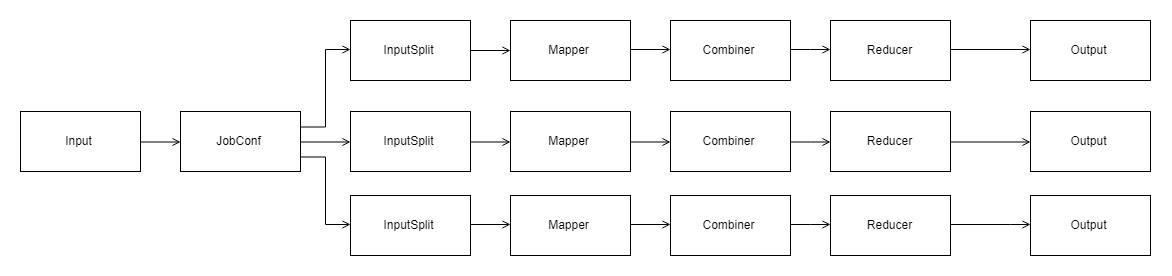
\includegraphics[scale=0.5]{05.wordcount_flowchart}
\caption{How Mapper and Reduce work}
\label{fig:mapreducefigure}
\end{figure}

\section{Who does what?}
Code: Dang Vinh Bao, Vu Hoang Linh
Report and misc.: Nguyen Thanh Long, Phung Duc Tuan

\end{document}
